\newpage
\section{LECTURE 8}

\subsection{Agenda}
\begin{itemize}
    \item Dynamic Programming
    \item Convexity
\end{itemize}

\subsection{Bellman's Principle}
\begin{itemize}
    \item Optimal control problems have an inherently sequential structure. 
    \item Past control inputs affect future states but future control inputs cannot affect past states. 
    \item Bellman's principle (i.e. The principle of optimality), states the consequences of this for optimal trajectories. 
    \item Sub-trajectories of optimal trajectories have to be optimal for the appropriately defined sub-problem.
\end{itemize}

\begin{figure}
    \centering
    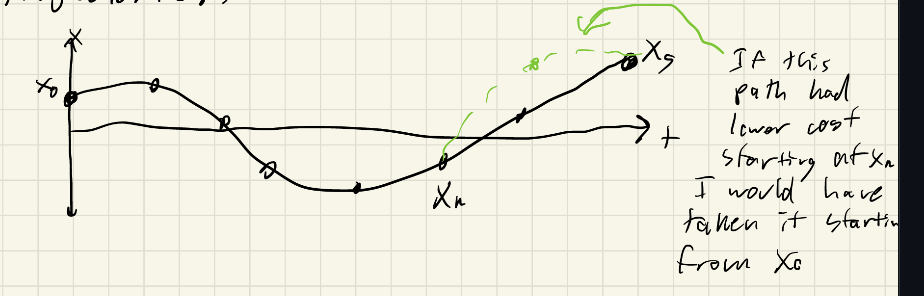
\includegraphics[width=0.4\linewidth]{L8_Images/F1.PNG}
    \caption{Bellman's Principle}
    \label{fig:l8f1}
\end{figure}

\subsection{Dynamic Programming}
\begin{itemize}
    \item Bellman's Principle suggests starting from the end of the trajectory and working backwards. 
    \item We've already seen hints of this in the Riccati equation, and in the co-state / multiplier equation from Pontryagin. 
    \item Define ``optimal cost-to-go'' a.k.a ``value function'' $V_N(x)$.
    \item Encodes the cost incurred starting from state $x$ at time $k$ if we act optimally. 
    \item For the LQR setting, we have: 
    \begin{align}
        V_N(x) = \frac{1}{2} x^T Q_N x = \frac{1}{2} x^T P_N x  
    \end{align}
    \item Now we can back up one time step, and compute $V_{N-1}(x)$:
    \begin{align}
        \min_u & \frac{1}{2} x_{N-1}^T Q x_{N-1} + \frac{1}{2} u^T R u + V_N (A_{N-1} x_{N-1} + B_{N-1} u) \\
        &= \min_u \frac{1}{2} u^T R u + \frac{1}{2} (A x_{N-1} + B_{N-1} u)^T Q_N  (A x_{N-1} + B_{N-1} u)
    \end{align}
    Since for the optimal action we have $\nabla_u $ of this cost $=0$, we have: 
\begin{align}
    u^T R_{N-1} + (A x_{N-1} + B_{N-1} u)^T Q B_{N-1} = 0 \\
    \implies u_{N-1} &= -(R_{N-1} + B_{N-1}^T Q_N B_{N-1})^{-1} B_{N-1}^T Q_N A_{N-1} x_{N-1} 
\end{align}
    We may define $K_{N-1}$ as $(R_{N-1} + B_{N-1}^T Q_N B_{N-1})^{-1} B_{N-1}^T Q_N A_{N-1}$ for convenience. 
    \item Plugging in $u=-Kx$ into our expression for $V_{N-1}(x)$, we have: 
    \begin{align}
        V_{N-1}(x) &= \frac{1}{2} x^T (Q_{N-1} + K_{N-1}^T R_{N-1} K + (A_{N-1} - B_{N-1} K_{N-1})^T Q_N (A_{N-1} - B_{N-1} K_{N-1}) ) x
    \end{align}
    We can define $P_{N-1} = (Q_{N-1} + K_{N-1}^T R_{N-1} K + (A_{N-1} - B_{N-1} K_{N-1})^T Q_N (A_{N-1} - B_{N-1} K_{N-1}) )$, such that:
    \begin{align}
        V_{N-1}(x) &= \frac{1}{2} x^T P_{N-1} x 
    \end{align}
    
    \item We now have a recursion in $K$ and $P$ that we can iterate until $k=1$. This is just the Riccati equation again. 
\end{itemize}

\subsubsection{Backward Dynamic Programming Algorithm}

\\
\noindent
\begin{algorithm}
	\caption{Backward DP Algorithm}
	\label{alg:bdp}
	\begin{algorithmic}[1]	
        \State $V_N(x) \gets l_N(x)$
        \State $K \gets N$
        \While {$K>1$} 
            \State $V_{k-1} = \min_u \big[ l(x,u) + V_k(f(x,u))\big]$ \Comment{The Bellman Equation.}
            \State $k \gets k-1$
        \EndWhile
	\end{algorithmic}
\end{algorithm}
\\

\begin{itemize}
    \item If we know $V_k(x)$, the optimal feedback policy is: 
    \begin{align}
        u_{k}(x) &= \arg\min_u \big[ l(x_k,u) + V_{k+1}(f(x_{k},u)) \big]
    \end{align}
    \item DP equations can be written equivalently in terms of action-value or $Q$ functions:
    \begin{align}
        S_k(x,u) &= l(x,u) + V_{k+1} (f(x,u)) \\
        \implies u_k(x_k) &= \arg\min_u S_k(x_k,u)
    \end{align}
    \item These are usually denoted $Q(x,u)$, be we will use $S$, since $Q$ is used in the LQR state cost as well. 
\end{itemize}

\subsubsection{The Curse}
\begin{itemize}
    \item DP is sufficient for a global optimum. 
    \item It is only tractable for simple problems, such as LQR problems or low-dimensional problems. 
    \item $V(x)$ stays quadratic for LQR problems, but becomes impossible to write down analytically for even simple non-linear problems. 
    \item Even if we could, the $\min_u S(x,u)$ will be non-convex, and possibly hard to solve on its own. 
    \item The cost of DP blows up with state dimension, due to the difficulty of representing $V(x)$. 
\end{itemize}

\subsubsection{Why do we care?}
\begin{itemize}
    \item Approximate DP, where $V(x)$, or $S(x,u)$ are reprsented with function approximators can work well. 
    \item Forms the basis of a lot of modern Reinforcement Learning. 
    \item DP generalizes to stochastic problems well, (just wrap everything in expectation operators), whereas Pontryagin's does not. 
\end{itemize}

\subsubsection{What are those Lagrange Multipliers?}
\begin{itemize}
    \item Recall Riccati derivation from QPs:
    \begin{align}
        \lambda_n &= P_n x_n \\
        P_n &= Q + A^T P_{n+1} (A-BK) \\
        &= Q + K^T R K + (A-BK)^T P_{n+1} (A-BK) \\
        V_n(x) &= \frac{1}{2} x^T P_n x \\
        \implies \lambda_n &= \nabla_x V_n(x)
    \end{align}
    \item The dynamics multipliers are the cost-to-go gradients! 
    \item Carries over to the general non-linear setting, beyond just LQR. 
\end{itemize}

\subsubsection{Example}
Remember to check out the lecture video for an example, where $\lambda_n$ from the QP matches $\nabla_x V_n(x)$ from DP. 

\subsection{Convex Model-Predictive Control}
\begin{itemize}
    \item LQR is very powerful, but often need to explicitly reason about constraints. 
    \item Often these are simple (ex. torque limits), and can be encoded as a convex set. 
    \item Constraints break the Riccati solution, but we can still solve the QP online. 
    \item Convex MPC has gotten extremely popular as computers have gotten faster. 
\end{itemize}

\subsubsection{Background: Convexity}
\begin{itemize}
    \item Convex Set: A line connecting any two points in the set is contained within the set.
    \item Standard examples:
    \begin{itemize}
        \item Linear subspaces ($Ax=b$). 
        \item Half-spaces, boxes, and polytopes ($Ax\leq b$). 
        \item Ellipsoids ($x^T P x \leq 1$).
        \item Cones ($||x_{2:n}||_2 \leq x_1$). This is called the second order cone, it's the usual ice-cream cone you're used to. 
    \end{itemize}
    \item Convex functions: A function $f(x): \matbb{R}^n \longrightarrow \mathbb{R}$ who's epigraph is a convex set. 
    \item Examples: 
    \begin{itemize}
        \item Linear $f(x) = c^T x$.
        \item Quadratic $f(x) = \frac{1}{2} x^T Q x + q^T x, \ni Q \geq 0$.
        \item Norms $f(x) = |x|$.
    \end{itemize}
    \item Convex Optimization Problem: Minimize a convex function over a convex set. 
    \item Examples:
    \begin{itemize}
        \item Linear Program (LP): Linear $f(x)$, linear $c(x)$.
        \item Quadratic Program (QP): Quadratic $f(x)$, linear $c(x)$. 
        \item Quadratically Constrained (QCQP): Quadratic $f(x)$, ellipsoid $c(x)$. 
        \item Second-order cone program (SOCP): Linear $f(x)$, cone $c(x)$. 
    \end{itemize}
    \item Convex problems don't have spurious local optima that satisfy the KKT. If you find a local KKT solution, you have the global optimum!
    \item Practically, Newton's method converges really fast and reliably (~5-10 iterations at maximum). 
    \item Can bound the solution time for real-time control.
\end{itemize}

\subsection{Convex MPC}
\begin{itemize}
    \item Think of this as "constrained LQR"
    \item Rememver from DP, if we have the cost-to-go, we can get $u_k$ by solving a one-step problem
    \begin{align}
    u_k &= \arg\min_u l(x_k, u) + V_{k+1}(f(x_k,u)) \\
    &= \arg\min_u \frac{1}{2} u^TR_k u + \frac{1}{2} (A_k x_k + B_k u)^TP_{k+1}(A_k x_k + B_k u)
    \end{align}
    \item We can add constraints on u to this one-step problem, but will perform poorly because $V_k(x)$ was computed without constraints.
    \item There's no reason I can't add more steps to the one-step problem:
    \begin{align}
        \min_{x_{1:H}, u_{1:H-1}} &\sum_{k=1}^{H-1} \frac{1}{2} x_k Q_k x_k + \frac{1}{2} u_k^T R_k u_k + x_H^T P x_H \\
        \ \ni \ x_k &\in X \\
        u_k &\in U
    \end{align}
    \item $H \leq N$ is called the "Horizon"
    \item With no additional constraints, MPC/"receediing horizon" exactly matches LQR for any H.
    \item Intuition: explicit constrained Optimization over the first H steps getting the state close enough to the origin/reference, so that the constraints are no longer active and LQR solution is valid farther into the futrue.
    \item In General:
    \begin{itemize}
        \item A good approximation of V(x) is important for good performance.
        \item Better V(x) $\Rightarrow$ shorter horizon will work.
        \item Longer H $\Rightarrow$ better performance, less reliance on quality of V(x) approximation.
    \end{itemize}
\end{itemize}

\subsection{Example}

\begin{figure}
    \centering
    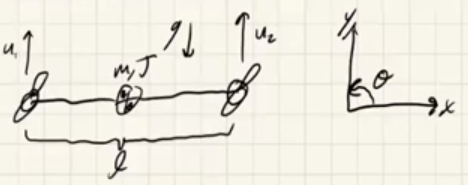
\includegraphics[width=0.4\linewidth]{L8_Images/F2.PNG}
    \caption{Planar Quadrotor}
    \label{fig:l8f2}
\end{figure}

\begin{itemize}
    \item Planar Quadrotor
    \begin{align}
        m \ddot x &= -(u_1 + u_2) \sin(\theta) \\
        m \ddot y &= (u_1 + u_2) \cos(\theta) - mg \\
        J \ddot \theta &= \frac{1}{2} l (u_2 - u_1)
    \end{align}
    \item Linearize about hover(approximate on angle, so it's right as long as the angle is small):
    \begin{align}
        & \Rightarrow u_1 = u_2 = \frac{1}{2} mg \text{ (cancel gravity)} \\
        & \Rightarrow 
        \begin{cases}
            \Delta \ddot x \approx -g \Delta \theta \\
            \Delta \ddot y \approx \frac{1}{m} (\Delta u_1 + \Delta u_2) \\
            \Delta \ddot \theta \approx \frac{1}{J} \frac{l}{2}(\Delta u_2 - \Delta u_1)
        \end{cases} \\
    \end{align}

    \begin{align}
        \begin{bmatrix}
            \Delta \dot x \\
            \Delta \dot y \\
            \Delta \dot \theta \\
            \Delta \ddot x \\
            \Delta \ddot y \\
            \Delta \ddot \theta \\
        \end{bmatrix} &= 
        \begin{bmatrix}
             &  &  & | &  &  &  \\
             & 0&  & | &  & I&  \\
             &  &  & | &  &  &  \\
            - & - & - & - & - & - \\
            0& 0& -g& | & & &  \\
            0& 0& 0& | & & 0&  \\
            0& 0& 0& | & & &  \\
        \end{bmatrix}
        \begin{bmatrix}
            \Delta  x \\
            \Delta  y \\
            \Delta \theta \\
            \Delta \dot x \\
            \Delta \dot y \\
            \Delta \dot \theta \\
        \end{bmatrix} + 
        \begin{bmatrix}
            0 & 0 \\
            0 & 0 \\
            0 & 0 \\
            - & - \\
            0 & 0 \\
            \frac{1}{m} & \frac{1}{m} \\
            -\frac{l}{2J} &\frac{l}{2J} 
        \end{bmatrix}
        \begin{bmatrix}
            \Delta  u_1 \\
            \Delta  u_2 \\
        \end{bmatrix} \\
        & \Rightarrow \dot X = AX + Bu
    \end{align}

    \item MPC Cost Function: 
    \begin{align}
        J = \sum_{k = 1}^H \frac{1}{2} (X_k - X_{ref})^T Q (X_k - X_{ref}) + \frac{1}{2} \Delta u_k^T R \Delta u_k + (X_H - X_{ref})^T P_H (X_H - X_{ref})
    \end{align}

    \item Remember to check out the example of this in the lecture video.
\end{itemize}

\subsection{Other MPC Examples}
\begin{figure}
    \centering
    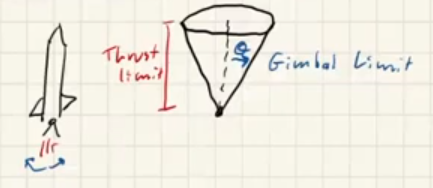
\includegraphics[width=0.4\linewidth]{L8_Images/F3.PNG}
    \caption{Rokcet Landing}
    \label{fig:l8f3}
\end{figure}
\begin{figure}
    \centering
    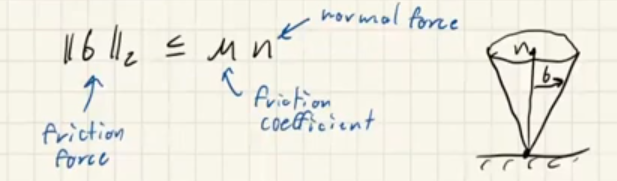
\includegraphics[width=0.4\linewidth]{L8_Images/F4.PNG}
    \caption{Legged robots friction cone}
    \label{fig:l8f4}
\end{figure}

\begin{figure}
    \centering
    
\includegraphics[width=0.2\linewidth]{L8_Images/F5.PNG}
    \caption{Four-sided pyramid}
    \label{fig:l8f5}
\end{figure}

\begin{itemize}
    \item Rocket Landing
    \begin{itemize}
        \item Thrust vector constraints are natually expressed as a cone! \cref{fig:l8f3}
        \item Mars landing + SpaceX use SOCP-based MPC with linearized dynamics
    \end{itemize}
    \item Legged Robots
    \begin{itemize}
        \item Contact forces must obey "friction cone" constraints.\cref{fig:l8f4}
        \begin{align}
            \Vert b \Vert_2 \leq \mu n
        \end{align}
        \item Cone is often approximated as a four-sided pyramid, so thee constraint is linear ($Ax \leq b$) \cref{fig:l8f5}
        \item MIT Cheetah and other quadropeds use QP-based MPC with linearized dynamics + friction pyramid.
    \end{itemize}
\end{itemize}

\subsection{What about Nonlinear Dynamics?}

\begin{itemize}
    \item Linear stuff often works well, so use it if you can.
    \item Nonlinear dynamics are risky because optimization problems are non-convex.
    \item No convergence guarentees.
    \item Can work well in practice, due to warm starting (solution doesn't change much at each itteration).
    \item Active area of research.
    \item Common in autonomous driving.
\end{itemize}